\chapter{Appendix} \label{chapter: Appendix}

\begin{code}[htpb]
    \centering
    \begin{tabular}{c}
    \begin{lstlisting}[language=ruby]
        apiVersion: apps/v1
        kind: DaemonSet
        metadata:
          name: green-daemon
          namespace: default
          labels:
            unikernel: "true"
        spec:
          selector:
            matchLabels:
              name: green-daemon
          template:
            metadata:
              labels:
                name: green-daemon
            spec:
              containers:
                - name: sayer
                  image: led-daemon
                  args:
                    - GREEN
              nodeSelector:
                  type: virtual-kubelet
                  raspberrypi: "true"
                  light:"GREEN"
              tolerations:
              - key: "virtual-kubelet.io/provider"
                operator: "Equal"
                value: "unikernel"
                effect: "NoSchedule"
  \end{lstlisting}
  \end{tabular}
  \caption{Green-daemon specification}\label{fig:green-daemon}
  \end{code}


  \begin{figure}
    \centering
    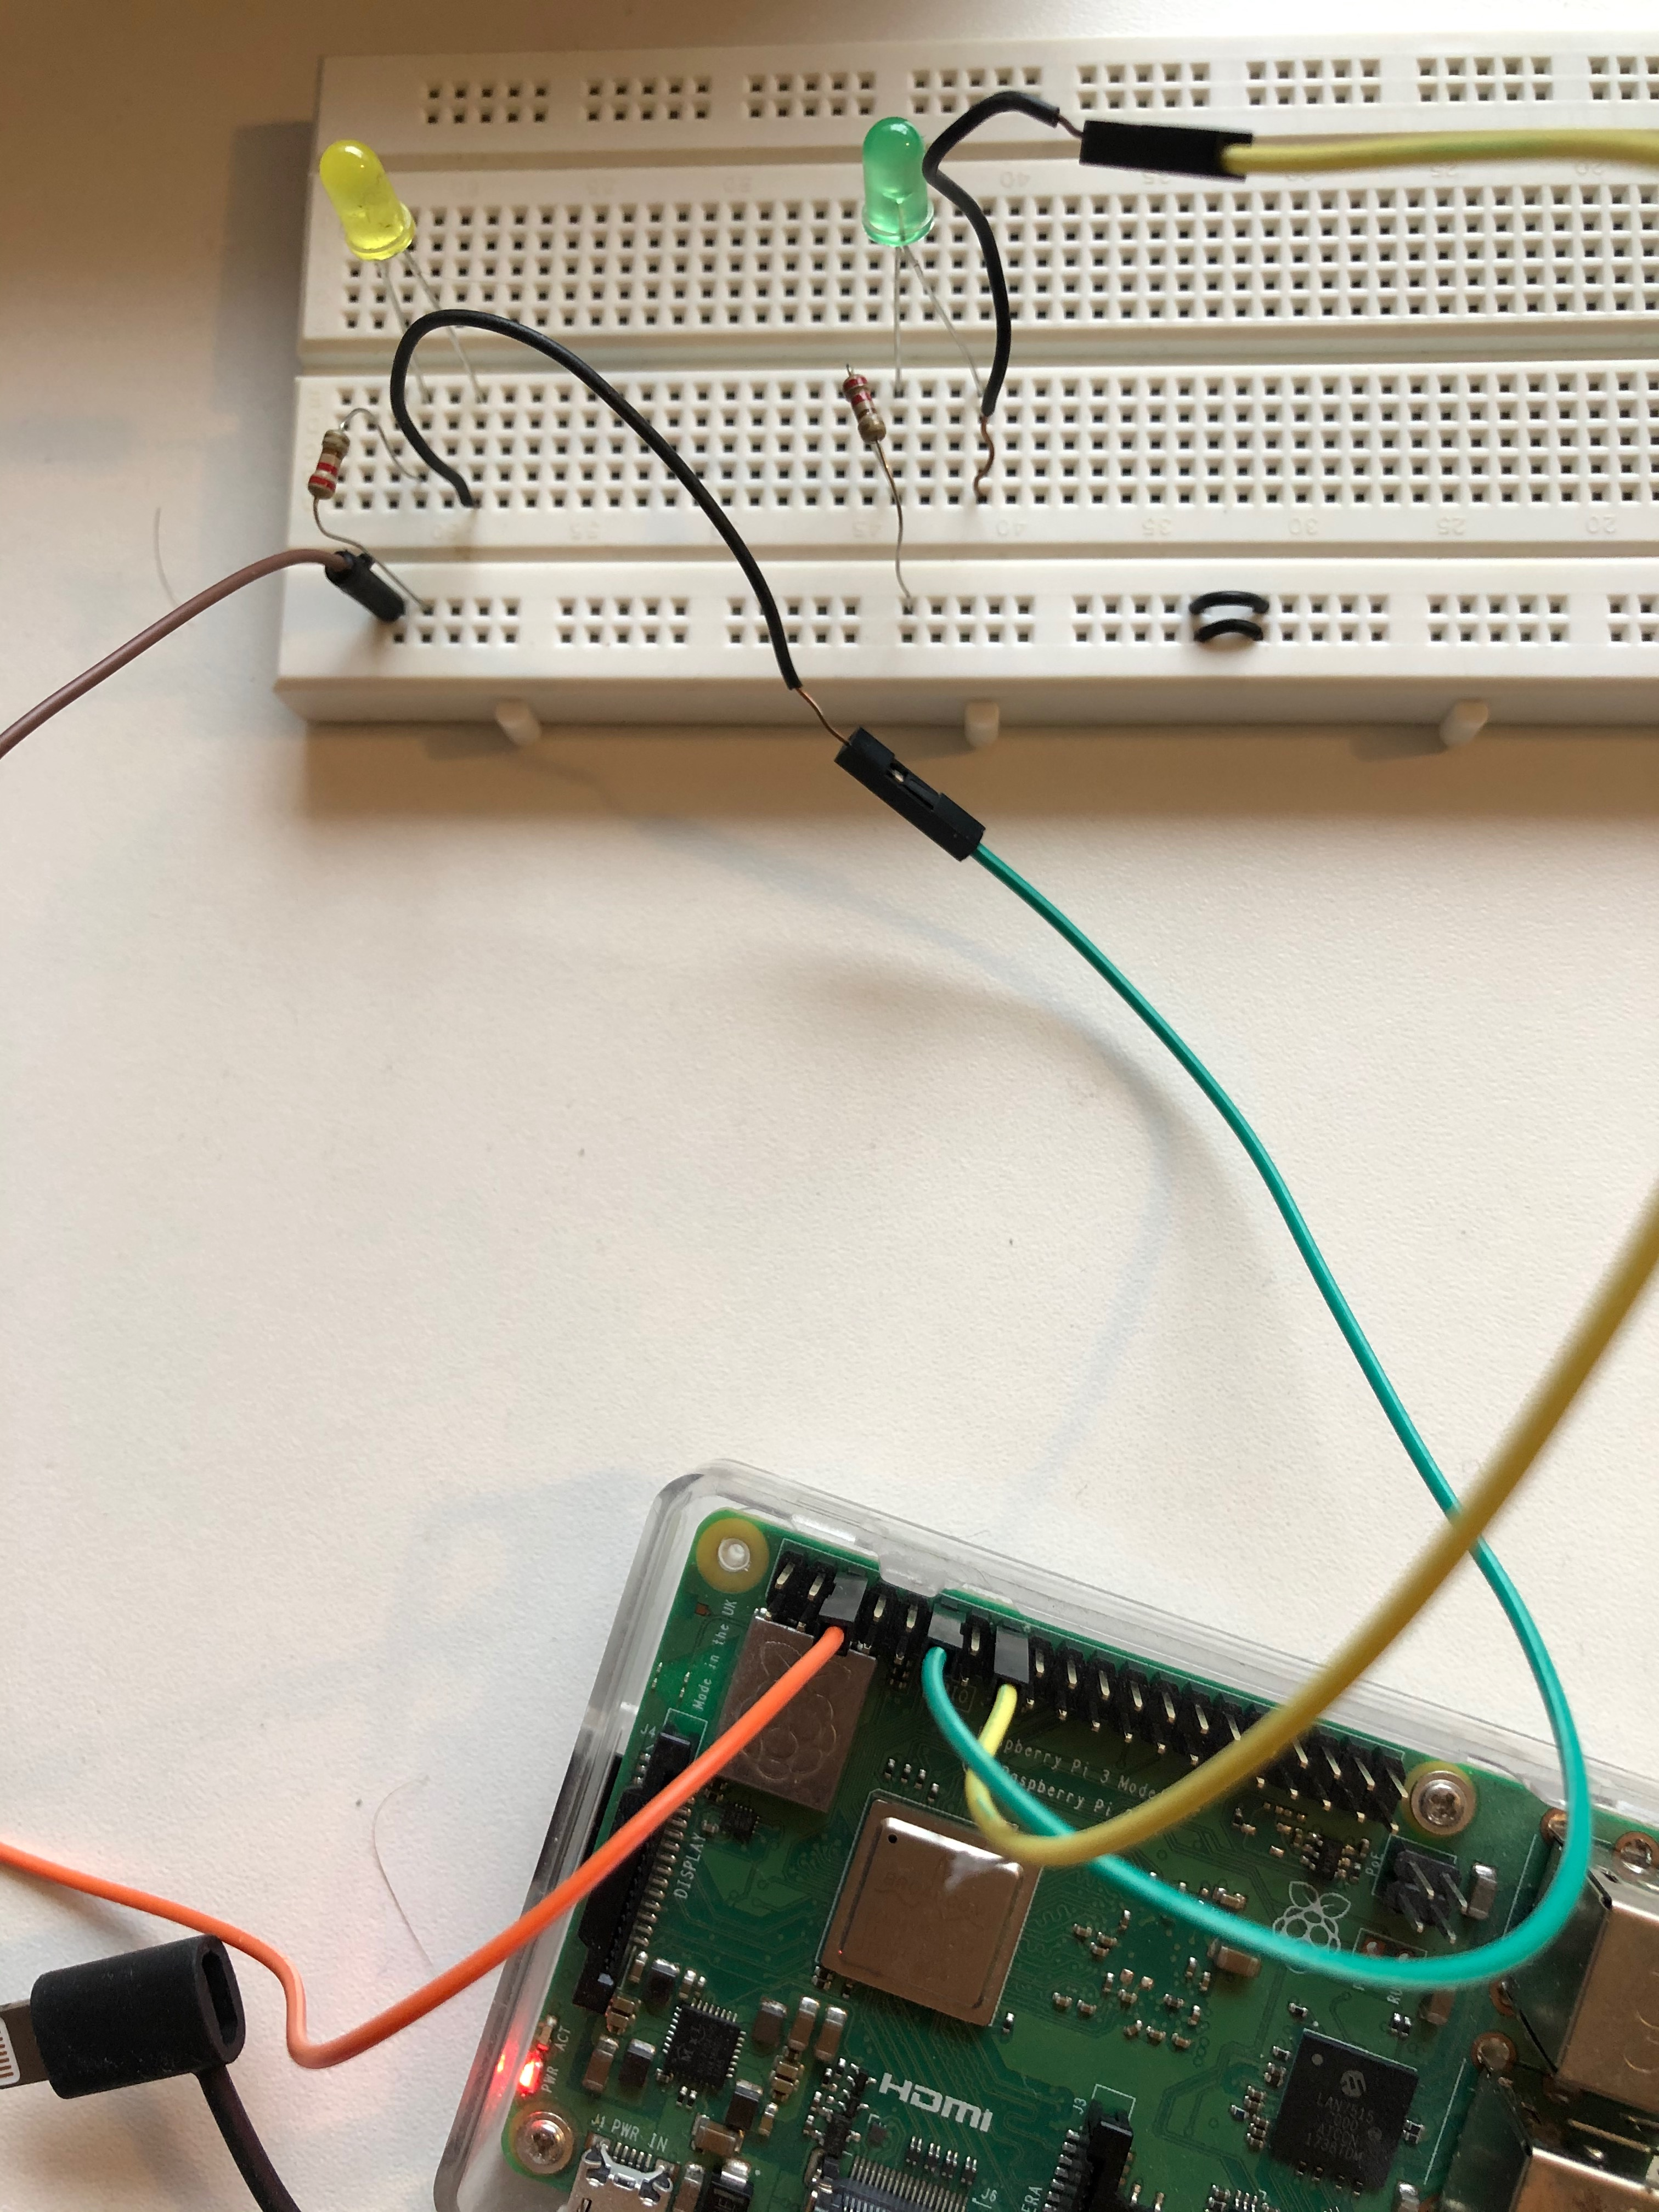
\includegraphics[width=0.9\textwidth]{rasp-running.jpeg}
    \caption{Physical wiring of \ref{fig:rpi-diagram}}
  \end{figure}
  